\documentclass[a4paper,10pt]{article}
\usepackage[utf8]{inputenc}
\usepackage{amsmath}
\usepackage{amsfonts}
\usepackage{amssymb}
\usepackage{algorithm}
\usepackage[noend]{algpseudocode}
\usepackage{program}
\usepackage{amsmath}
\usepackage{graphicx}
\usepackage[T1]{fontenc}
\usepackage{eso-pic}
\usepackage{gensymb}
\usepackage{listings}
\usepackage{float}

\newcommand{\BackgroundPic}{\put(-4,0){\parbox[b][\paperheight]{\paperwidth}{\centering
\includegraphics[width=\paperwidth,height=\paperheight]{nat-farve.pdf}}}}

\algnewcommand\True{\textbf{true}\space}
\algnewcommand\False{\textbf{false}\space}
\algdef{SE}[SUBALG]{Indent}{EndIndent}{}{\algorithmicend\ }%
\algtext*{Indent}
\algtext*{EndIndent}

\begin{document} 
	\AddToShipoutPicture*{\BackgroundPic}
	
	\begin{titlepage}
		\thispagestyle{empty}
		\vspace*{5cm}
		\begin{center}
			\Huge \textbf{Diskret Matematik og Algoritmer} \\
			\LARGE \textbf{Aflevering 6i (Genaflevering)} \\
		\end{center}
		\vspace*{3.5cm}
		\begin{flushleft}
			
		\begin{table}[h!]
			\begin{tabular}{lll}
				Adam Ingwersen,& \\ GQR701 \\
			\end{tabular}
		\end{table}
			
			
			\vspace{3mm}
			\vspace{3mm}
			Datalogisk  Institut\\
			Københavns Universitet\\
			\vspace{3mm}
			\today\\
			%\vspace*{0.5cm}
			
		\end{flushleft}
	\end{titlepage}

	\title{5g}
	\author{ncog}
	
	\newpage

\newpage

\section*{Del 1}
Vi betragter Fibonaccitallene og disses definition; $F_{0} = 0, F_{1} = 1$ og derefter:
$$
F_{n} = F_{n-1} + F_{n-2} \quad \forall n \geq 2
$$
\subsection*{(1)}
Ved præsentation af induktionsbevis fremvises først og fremmest et basis-step, der efterviser, at $P(n_{0})$ gælder. Herefter gøres en antagelse om $P(n)$. Ud fra denne antagelse forsøges det at vise, at $P(n) \implies P(n+1)$ er en tautologi - dette er sandt når implikationspilen er sand. 
\newline
\subsubsection*{Basis-step}
$$
P(1): \quad F_{2} = F_{1} + F_{0} = 2 \leq 2^{1} = 2
$$
\subsubsection*{Induktions-step}
Vi gør os nu en antagelse om $P(k)$:
$$
P(k): \quad F_{k} \leq 2^{k}
$$

Nu skal det vises, at $P(k+1)$ gælder givet definitionen af Fibonacci-sekvensen defineret i Del 1:
$$
P(k+1): \quad F_{k+1} = F_{k} + F_{k-1} \leq 2^{k+1} = 2 \cdot 2^{k} = F_{k} + F{k}
$$
Givet den rekursive definition af $F_{n}$ gælder det, at:
$$
P(k+1): \quad F_{k} + F_{k-1} \leq F_{k} + F_{k}
\quad \quad \forall k \in \mathbb Z^{+} \quad \quad Q.E.D.
$$

Altså, er $P(k+1)$ sand. Efter princippet for matematisk induktion gælder det, at $P(n)$ er sand for alle $n \geq 1$

\subsection*{(2)}
\subsubsection*{Basis-step}
$$
P(6): \quad F_{6} = 8 \geq \frac{3}{2}^{5} \approx 7,6
$$
Base-case, $P(6)$, er sand. Nu skal det vises, at nedenstående gælder. 
$$
F_{n} \geq (\frac{3}{2})^{n-1} \quad \forall n \in \{6, 7, 8,...\}
$$

\subsubsection*{Induktions-step}
Det vises, at også $P(7)$ sand:
$$
P(7) : F_{7} = 13 \geq \frac{3}{2}^6 \approx 11,39
$$
Givet, $P(6)$ og $P(7)$ sand, antages $P(k-1)$ samt $P(k)$ sand, således at:

\begin{equation}
\begin{aligned}	
F_{k+1}	 	= 		& F_{k} + F_{k-1} \\
			\geq	& (\frac{3}{2})^{k-1} + (\frac{3}{2})^{k-2} \\
			=		& (\frac{3}{2})^{k-2} \cdot (\frac{3}{2} + 1) \\
			>		& (\frac{3}{2})^{k-2} \cdot (\frac{3}{2})^{2} \\
			=		& (\frac{3}{2})^{k} \\
			\implies & F_{k+1} \geq (\frac{3}{2})^{k} \quad Q.E.D.
\end{aligned}
\end{equation}

Hermed vist. Det bemærkes, at vores basis-step bryder sammen for $n < 6$ - hvorfor det gælder:
$$
F_{n+1} \geq (\frac{3}{2})^{n} \quad \forall n \in \{6, 7, 8,...\}
$$

\subsection*{(3)}

For at bestemme tids-kompleksiteten af Fibonacci-sekvensen, skal vi undersøge, hvor mange led der skal udregnes før et vilkårligt $F_{n}$ er identificeret. Givet den rekursive definition af $F_{n}$, skal vi finde en funktion der tilfredsstiller:
$$
F_{1} = 1 \quad \wedge \quad
F_{n} = F_{n-1} + F_{n-2}
$$

Vi ved, at $F_{n}$ er $\Omega (\frac{3}{2}^{n-1})$, samt $O (2^{n})$. Dette er $F_{n}$'s lower- hhv. upper-bound. Mellem disse to funktioner findes en $\Theta$-repræsentation af $F_{n}$. For at finde køretiden af $log_{2}F_{n}$, tages 2-tals logaritmen til de to udtryk, hvor ulighedstegn anvendes for at indikere, at $log_{2}F_{n}$ ligger imellem:

\begin{equation}
\begin{aligned}	
\Omega (log_{2}\frac{3}{2}^{n-1}) \leq log_{2}F_{n} \leq  O (log_{2}2^{n}) \\
\implies k \cdot (n-1) \leq log_{2}F_{n} \leq n
\end{aligned}
\end{equation}

Altså, ligger $log_{2}F_{n}$ mellem to lineære funktioner af n, således at det asymptotisk gælder, at $log_{2}F_{n}$ er $\Theta(n)$. Logaritmen til Fiboancci-sekvensen har konstant tids-kompleksitet, hvorved vi kan udlede, at tidskompleksiteten af Fibonacci-sekvensen må være non-lineær.  

\begin{figure}[H]
\centering
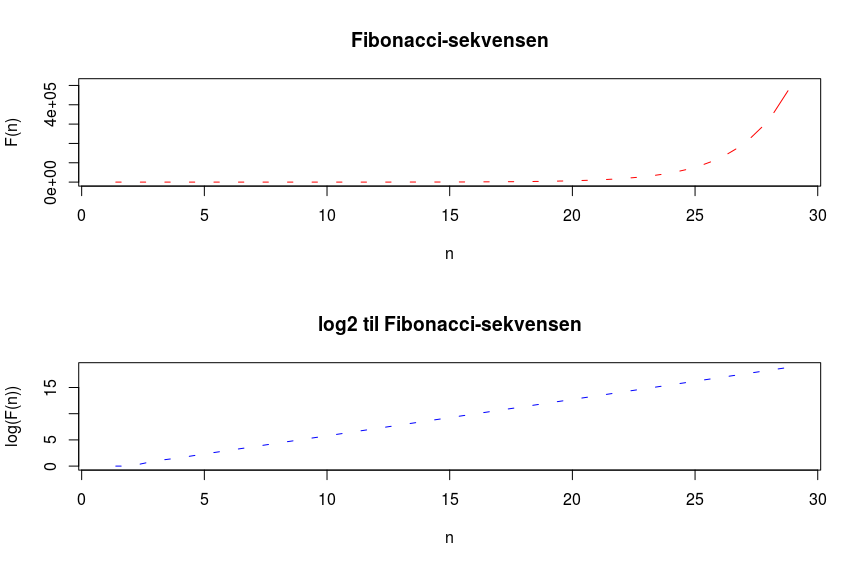
\includegraphics[scale = 0.5]{fibSeq.png}
\end{figure}

\section*{Del 2}
\subsection*{(1)}
Algoritmen MUL bestemmer hvorvidt to positive tal, $a,\quad b \in \mathbb Z^{+}$, er ligeligt divisible. Variablen y tæller antallet af gange, a kan divideres med b - eller rettere, hvor mange gange b går op i a. Det formodes, at der med illustrative eksempler menes et par repræsentative eksempler af algoritmens virken:
\begin{equation}
\begin{aligned}	
MUL(10, 5)		\implies	& x = 10, y = 0 \rightarrow x = 10-5 = 5, y = 1 \rightarrow  x = 5-5 = 0, y = 2 \\
				\implies	& x = 0, y = 2, RETURN = TRUE \\
MUL(11, 6)		\implies 	& x = 11, y = 0 \rightarrow  x = 11-6 = 5, y = 1 \rightarrow END LOOP: x \ngeq b \\
				\implies	& x = 5, y = 1, RETURN = FALSE
\end{aligned}
\end{equation}

\subsection*{(2)}
\subsubsection*{Basis-step}
\begin{equation}
\begin{aligned}	
x_{0} 					= & a \\
y_{0}					= & 0 \\
x_{0} +b\cdot y_{0} 	= & a \\
\implies x_{0} 			= & a
\end{aligned}
\end{equation}
$P(0)$ er altså sand. 

\subsubsection*{Induktions-step}
Med udgangspunkt i $P(0)$ antager vi, at $P(k)$ er sand, sådan at:
$$
P(k): \quad x_{k} + b \cdot y_{k} = a \iff x_{k} = a - b \cdot y_{k}
$$
Det skal eftervises, at der efter $n$ gennemløb af while-løkken gælder:
\begin{equation}
\begin{aligned}	
x_{n} + b\cdot y_{n} = a
\end{aligned}
\end{equation}

For at vise det generelle tilfælde, betragtes udtrykket ved $n+1$'te gennemløb:
\begin{equation}
\begin{aligned}	
x_{n+1} + b \cdot y_{n+1} = a
\end{aligned}
\end{equation}

Vi ved, at $y_{k+1} = y_{k} + 1$ pr. definition. Det ses, at der må gælde:
\begin{equation}
\begin{aligned}	
x_{n+1} = x_{n} - b
y_{n+1} = y_{n} + 1
\end{aligned}
\end{equation}

Lighederne i (7) substitueres ind i (6), hvorved vi får:
\begin{equation}
\begin{aligned}	
x_{n+1} b \cdot y_{n+1} = x_{n} - b + b \cdot (y_{n} + 1) \\
x_{n+1} b \cdot y_{n+1} = x_{n} - b + b \cdot y_{n} + b \\
x_{n+1} b \cdot y_{n+1} = x_{n} + b \cdot y_{n} = a
\end{aligned}
\end{equation}

Hermed er det vist, induktivt, at $x_{n} + b\cdot y_{n} = a$ i det generelle tilfælde.

\subsection*{(3)}

Algoritmen terminerer med FALSE/TRUE. For at dette lader sig gøre, kræves det at $b \geq x \geq 0$ i pseudokoden. Det bemærkes, at vi kan repræsentere $a$ som $ a = n \cdot b + r$, hvor $b > r \geq 0$. I udtrykket er $r$ en rest - vi kan således repræsentere algoritmens udfald (FALSE/TRUE) vhja. $r$, altså to tilfælde: 
\begin{equation}
\begin{aligned}	
b\mid a \implies r = 0 \quad \vee \quad b \nmid a
\end{aligned}
\end{equation}

Lad det $q$'te iteration af while-løkken være den terminerende (sidste) iteration. Vi bruger, at $y$ vokser med 1 pr. iteration, og må ved den $q$'te iteration være $q$:
\begin{equation}
\begin{aligned}	
x_{q}  b \cdot y_{q} = a\\
x_{q} + b \cdot y_{q} = q \cdot b + r \\
x_{q} = q \cdot b + r - b \cdot y_{q} \\
x_{q} = q \cdot b + r - b \cdot q \\
x_{q} = r
\end{aligned}
\end{equation}

Altså må algoritmen terminere, og derved returnere et af de to mulige udfald, FALSE/TRUE.

\newpage

\section*{Bilag}
\lstinputlisting[language=R]{fibSeq.R}

\end{document}